\documentclass[9pt,a4paper]{extarticle}


	\usepackage[margin=5em,bottom=8em]{geometry}


%1 est la marge gauche
%2 est la marge en haut
%3 est la marge droite
%4 est la marge en bas
%5 fixe la hauteur de l'entête
%6 fixe la distance entre l'entête et le texte
%7 fixe la hauteur du pied de page
%8 fixe la distance entre le texte et le pied de page
%------------------------------Packages généraux------------------------------

\usepackage[english]{babel}
\usepackage[T1]{fontenc}
\usepackage{ae}
\usepackage[utf8]{inputenc}
\usepackage{scrextend}
\usepackage{diagbox}
\usepackage{hyperref}
 \hypersetup{
    colorlinks = true,
    linkcolor=black,
    urlcolor = black
    }
%-------------------------Mathématiques------------------------------
\usepackage{amsmath}
\usepackage{amssymb}
\usepackage{amsthm}
\usepackage{amsfonts}
\usepackage{eucal}
\newcommand\independent{\protect\mathpalette{\protect\independenT}{\perp}}
\def\independenT#1#2{\mathrel{\rlap{$#1#2$}\mkern2mu{#1#2}}}
%-----------------------Codes et algorithmes--------------------------
\usepackage{algorithm}
%\usepackage{algorithmic}
%\usepackage{clrscode3e}
\usepackage[noend]{algpseudocode}
%\newcommand{\pushline}{\Indp}% Indent
%\newcommand{\popline}{\Indm\dosemic}% Undent
%\newcommand{\nonl}{\renewcommand{\nl}{\let\nl\oldnl}}%


%------------------------------Graphics------------------------------

\usepackage{graphicx}
\usepackage{fancyhdr}
\usepackage{fancybox}
\usepackage{color}
\usepackage{pgf, tikz}
\usetikzlibrary{arrows, automata}
%\usepackage{slashbox}

%------------------Sub-sections--------%
\usepackage{titlesec}
\usepackage{hyperref}
\usepackage{comment}
\usepackage{qrcode}
\usepackage{subcaption}
\usepackage{hyperref}
               
 \hypersetup{
    colorlinks = true,
    linkcolor=black,
    urlcolor = black
    }
    
\newenvironment{solution}
    {%\begin{center}
    %\begin{tabular}{|p{0.9\textwidth}|}
    %\hline\\
    \color{red}
    }
    { 
    %\\\\\hline
    %\end{tabular} 
    %\end{center}
    \color{black}
    }
    
\newcommand{\blue}[1]{\textcolor{blue}{#1}}
\newcommand{\indep}{\rotatebox[origin=c]{90}{$\models$}}

\newenvironment{rcases}
  {\left.\begin{aligned}}
  {\end{aligned}\right\rbrace}
\newif\ifhideproofs
\hideproofstrue %uncomment to hide proofs

\ifhideproofs
\usepackage{environ}
\NewEnviron{hide}{}
\let\solution\hide
\let\endsolution\endhide
\fi

\title{{\bf INFO8006 Introduction to Artificial Intelligence}\\[1em]
Reasoning under uncertainty II}
\date{}
%------------------------------Début du document------------------------------
\begin{document}
\maketitle
\vspace{-4em}
%------------------------------Page de garde------------------------------

  \section*{Learning outcomes} 
      At the end of this exercise session you should be able to:
      \begin{itemize}
          \item Define and build a Bayesian network
          \item Compute probabilities in the context of a simple Bayesian network
          \item Apply variable elimination for inference
          %\item Explain the following approximate inference algorithm: ancestral sampling and rejection sampling; Likelihood weighting; Gibbs sampling.
      \end{itemize}
\section*{Exercise 1: Bag of coins}
We have a bag of three biased coins a, b, and c with probabilities of coming up heads
of 20\%, 60\%, and 80\%, respectively. One coin is drawn randomly from the bag (with equal
probability of drawing each of the three coins), and then the coin is flipped three times to
generate the outcomes $X1$, $X2$, and $X3$.
\begin{enumerate}
    \item Draw the Bayesian network corresponding to this setup and define the necessary CPTs.
    \begin{solution}
    \\
    We define the following random variables:
    \begin{itemize}
        \item $Y \quad \text{Dom}_Y = \{a, b, c\}$: The coin drawn from the bag.
        \item $X_1 \quad \text{Dom}_{X_1} = \{h, t\}$: The realisation of the first coin toss.
        \item $X_2 \quad \text{Dom}_{X_2} \{h, t\}$: The realisation of the second coin toss.
        \item $X_3 \quad \text{Dom}_{X_3} \{h, t\}$: The realisation of the third coin toss.
    \end{itemize}
    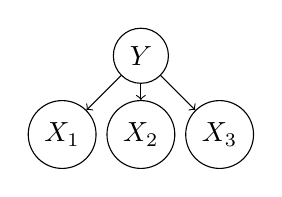
\begin{tikzpicture}[->]
    \node[circle, draw] (Y) at (0, 0) {$Y$};
    \node[circle, draw] (X1) at (-1, -1) {$X_1$};
    \node[circle, draw] (X2) at (0, -1) {$X_2$};
    \node[circle, draw] (X3) at (1, -1) {$X_3$};
    \draw (Y) -> (X1);
    \draw (Y) -> (X2);
    \draw (Y) -> (X3);
    \end{tikzpicture}
    \\
    \begin{table}[H]
        \centering
        \begin{tabular}{|c|ccc|}
    \hline
       $y$  & $a$ & $b$ & $c$ \\\hline
         & $\frac{1}{3}$& $\frac{1}{3}$& $\frac{1}{3}$\\ \hline
    \end{tabular}
    \caption{$P(Y = y)$}
    \end{table}
    
    \begin{table}[H]
        \centering
        \begin{tabular}{|c|ccc|}
    \hline
       \backslashbox{$x$}{$y$}  & $a$ & $b$ & $c$ \\\hline
        $h$ & $0.2$ & $0.6$ & $0.8$\\ \hline
        $t$ & $0.8$ & $0.4$ & $0.2$\\ \hline
    \end{tabular}
    \caption{$P(X_1 = x|Y = y)$}
    \end{table}
    
    \end{solution}
    \item Calculate which coin was most likely to have been drawn from the bag if the observed
flips come out heads twice and tails once.
\begin{solution}
\begin{align*}
    \hat{y} &= \arg\max_y P(y|h, h, t)\\
    &= \arg\max_y 3\times P(y|X_1 = h, X_2 = h, X_3 = t)\\
    &= \arg\max_y \frac{P(y, X_1 = h, X_2 = h, X_3 = t)}{P(X_1 = h, X_2 = h, X_3 = t)}\\
    &= \arg\max_y P(y, X_1 = h, X_2 = h, X_3 = t)\\
     &= \arg\max_y P(X_1 = h|y) P(X_2 = h|y) P(X_3 = t|y)P(y)\\
     &=\arg\max_y P(X_1 = h|y) P(X_2 = h|y) P(X_3 = t|y)\\
     &=\begin{rcases}
    y=a &: 0.2^2\times 0.8 = 0.032 \\
    y=b &: 0.6^2\times 0.4=0.144 \\
    y=c &: 0.8^2 \times 0.2=0.128
\end{rcases}
\text{$\hat{y} = b$}\\
\end{align*}
\end{solution}
\end{enumerate}
\section*{Exercise 2: Handedness (AIMA, Ex: 14.6)}
Let $H_x$ be a random variable denoting the handedness of an individual $x$, with possible
values $l$ or $r$. A common hypothesis is that left- or right-handedness is inherited by a simple
mechanism; that is, perhaps there is a gene $G_x$, also with values $l$ or $r$, and perhaps actual
handedness turns out mostly the same (with some probability $s$) as the gene an individual
possesses. Furthermore, perhaps the gene itself is equally likely to be inherited from either
of an individual’s parents, with a small nonzero probability $m$ of a random mutation flipping
the handedness.
\begin{enumerate}
    \item Which of the three networks in Figure \ref{fig:b_net} claim that\\ $P(G_{father},G_{mother},G_{child}) =
P(G_{father} )P(G_{mother} )P(G_{child} )$?
\begin{solution}
$c.$
\end{solution}
    \item Which of the three networks make independence claims that are consistent with the
hypothesis about the inheritance of handedness?
\begin{solution}
$a$ and $b$ ($b$ does not claim any independence).
\end{solution}
    \item Which of the three networks is the best description of the hypothesis?
    \begin{solution}
    $a.$
    \end{solution}
    \item Write down the CPT for the Gchild node in network (a), in terms of $s$ and $m$.
    \begin{table}[H]
        \centering
        \begin{tabular}{|c|c|c|}
        \hline 
           \backslashbox{$g_m$}{$g_f$}  & $l$ & $r$ \\ \hline
            $l$ & $1-m$ & $0.5$\\ \hline
            $r$ & $0.5$ & $m$\\ \hline
        \end{tabular}
        \caption{$P(\mathcal{G}_c = l|g_f, g_m)$} 
        \label{tab:my_label}
    \end{table}
    \item Suppose that $P(G_{father} =l) = P(G_{mother} =l) = q$. In network (a), derive an expression
for $P(G_{child} =l)$ in terms of $m$ and $q$ only, by conditioning on its parent nodes.
\begin{solution}
\begin{align}
    P(G_{child} = l) &= \sum_{g_m}\sum_{g_f} P(G_{child} = l, g_m, g_f)\\
    &=\sum_{g_m}\sum_{g_f} P(G_{child} = l| g_m, g_f)P(g_m)P(g_f)\\
    &= q^2(1-m) + 0.5q(1-q) + 0.5q(1-q) + (1-q)^2m\\
    &= q + m -2qm
\end{align}
\end{solution}
    \item Under conditions of genetic equilibrium, we expect the distribution of genes to be the
same across generations. Use this to calculate the value of q, and, given what you know
about handedness in humans, explain why the hypothesis described at the beginning of
this question must be wrong.
hypothesis about the inheritance of handedness?
\begin{solution}
$P(G_{child} = l) = P(G_{mother} = l) = P(G_{father} = l) \Leftrightarrow q = q + m -2qm $ and so $q=0.5$ which is not realisitic.
\end{solution}
\end{enumerate}

\begin{figure}
\begin{subfigure}{.3\linewidth}
\centering
\includegraphics[width=1.\textwidth]{figures/handedness1.eps}
\caption{}
\label{fig:sub1}
\end{subfigure}%
\begin{subfigure}{.3\linewidth}
\centering
\includegraphics[width=1.\textwidth]{figures/handedness2.eps}
\caption{}
\label{fig:sub1}
\end{subfigure}%
\begin{subfigure}{.3\linewidth}
\centering
\includegraphics[width=1.\textwidth]{figures/handedness3.eps}
\caption{}
\label{fig:sub1}
\end{subfigure}%
\caption{Possible Bayesian Networks of handedness inheritance}
\label{fig:test}
\end{figure}

\section*{Exercise 3: D-separation}
You are advised to take a look at d-separation before doing this exercise: \url{http://web.mit.edu/jmn/www/6.034/d-separation.pdf}.
\begin{figure}[H]
    \centering
    \includegraphics[width=1.\textwidth]{figures/pearl-bn-example.png}
    \caption{Bayesian Network of metastatic cancer}
    \label{fig:pearl-b-net}
\end{figure}
Consider the Bayesian network of Figure \ref{fig:pearl-b-net}, which, if any, of the following are asserted by the network structure ?
\begin{enumerate}
    \item $P(b, c) = P(b)P(c)$
    \item $P(b, c|a) = P(b|a)P(c|a)$
    \item $P(b, c| a, d) = P(b|a, d) P(c|a, d)$
    \item $P(c|a, d, e) = P(c|a, b, d, e)$
    \item $P(b, e|a) = P(b|a)P(e|a)$
    \item $P(b, e) = \sum_{a \in A, c \in C, d \in D} P(a) P(b|a) P(c|a) P(e|c) P(d|b, c)$
\end{enumerate}
\begin{solution}
\begin{enumerate}
    \item $B \indep C$? False.
    \item $B \indep C|A$? True.
    \item $B \indep C|A, D$? False.
    \item $B \indep C|A, D, E$ ? False (Markov blanket).
    \item $B \indep E | A$ ? True.
    \item $P(b, e) = \sum_{a \in A, c \in C, d \in D} P(a, b, c, d, e) = \sum_{a \in A, c \in C, d \in D} P(a) P(b|a) P(c|a) P(e|c) P(d|b, c) $, so it is correct.
\end{enumerate}
\end{solution}

$\star$ Use inference by variable elimination to compute $P(E|a, b)$.
\begin{solution}
\begin{align}
    P(E|a, b) &= \frac{1}{\alpha} \sum_{c, d} P(a, b, c, d, E)\\
    &=\frac{1}{\alpha} \sum_{c, d} P(a)P(b|a)P(c|a)P(d|b, c)P(E|c)\\
    &=\frac{1}{\alpha} P(a)P(b|a) \sum_{c}P(c|a)P(E|c)\sum_d P(d|b,c)
\end{align}
We define the initial factors as:
$F_1 = P(A=a)$, $F_2 = P(B=b|A=a)$, $F_3(C) = P(C|A=a)$, $F_4(C, D) = P(D|B=b, C)$, $F_5(E, C)P(E|C)$.
And then we compute:
$F_6(C) = \sum_d F_4(C, d)$, then $F_7'(C, E) = F_3(C)\times F_5(E, C)\times F_6(C)$ and $F_7(E) = \sum_c F_7'(c, E)$, then $F_8(E) = F_1 \times F_2 \times F_7(E)$, finally $P(E|a, b) = \frac{F_8(E)}{\sum_e F_8(e)}$
\end{solution}
% \section*{Exercise 4: Quiz }
% \begin{enumerate}
%     \item What is the Markov Blanket of a node ?
%     \item Fill in the Prior Sampling algorithm of Figure $\ref{fig:prior_sampling}$.
%     \item Why is Rejection sampling inefficient ?
%     \item Fill in the Gibbs Sampling algorithm of Figure $\ref{fig:gibbs_weighting}$.
% \end{enumerate}
% \begin{figure}[h]
%     \centering
%     \includegraphics[width=.6\textwidth]{figures/prior_sampling.png}
%     \caption{Incomplete Prior Sampling Algorithm}
%     \label{fig:prior_sampling}
% \end{figure}
% \begin{figure}[h]
%     \centering
%     \includegraphics[width=.6\textwidth]{figures/gibbs_weighting.png}
%     \caption{Incomplete Gibbs Sampling Algorithm}
%     \label{fig:gibbs_weighting}
% \end{figure}
\section*{Exercise 5: Car Diagnosis (AIMA, Ex: 14.8)}
\begin{figure}[h]
    \centering
    \includegraphics[width=.6\textwidth]{figures/car-starts.eps}
    \caption{A Bayesian network describing some features of a car’s electrical system and engine. Each variable is Boolean, and the true value indicates that the corresponding aspect of the vehicle is in working order.}
    \label{fig:car_bnet}
\end{figure}
Consider the network for car diagnosis shown in Figure \ref{fig:car_bnet}.
\begin{enumerate}
    \item Extend the network with the Boolean variables IcyWeather and StarterMotor.
    \begin{solution}
    IcyWeather is not caused by any of the car-related variables, so needs no parents. It directly affects the battery and the starter motor. StarterMotor is an additional precondition for Starts. The new network is shown in Figure \ref{fig:ext_car_bnet}.
    \begin{figure}[h]
        \centering
        \includegraphics[width=.9\textwidth]{figures/car_bnet_full.png}
        \caption{Extended Bayesian Network}
        \label{fig:ext_car_bnet}
    \end{figure}
    \end{solution}
    \item Give reasonable conditional probability tables for all the nodes.
    \begin{solution}
    Reasonable probabilities may vary a lot depending on the kind of car and perhaps the personal experience of the assessor. The following values indicate the general order of magnitude and relative values that make sense:
    \begin{itemize}
        \item  A reasonable prior for IcyWeather might be $0.05$ (perhaps depending on location and season).
        \item   $P(Battery|IcyWeather)=0.95,P(Battery|\lnot IcyWeather)=0.997$.
        \item   $P(StarterMotor|IcyWeather) = 0.98$, $P(Battery|\lnot IcyWeather) = 0.999$.
        \item   $P (Radio|Battery) = 0.9999, P (Radio|\lnot Battery) = 0.05$.
        \item   $P (Ignition|Battery) = 0.998, P (Ignition|\lnot Battery) = 0.01$.
        \item   $P (Gas) = 0.995$.
        \item   $P(Starts|Ignition,StarterMotor,Gas) = 0.9999, other entries 0.0$.
        \item   $P(Moves|Starts) = 0.998$.
    \end{itemize}
    \end{solution}
    \item How many independent values are contained in the joint probability distribution for eight Boolean nodes, assuming that no conditional independence relations are known to hold among them?
    \begin{solution}
    With 8 Boolean variables, the joint has $28 - 1 = 255$ independent entries.
    \end{solution}
    
    \item How many independent probability values do your network tables contain?
    \begin{solution}
    Given the topology shown in Figure S14.1, the total number of independent CPT entries is $1+2+2+2+2+1+8+2= 20$.
    \end{solution}
\end{enumerate}
\section*{Exercise 6 $\star$: Green Party President bis (Berkeley Spring 2014) }
Consider the following Bayesian network.
\begin{figure}[H]
    \centering
    \includegraphics{figures/GPP_bnet.pdf}
    \caption{Green Party President Bayesian Network}
    \label{fig:gpp_net}
\end{figure}
\begin{table}[h]
    \centering
    \begin{tabular}{|c|c|c|}
    \hline
         & $g$ & $\lnot g$ \\    \hline
        $P(G)$ & $0.1$ & $0.9$ \\    \hline
    \end{tabular}

    \begin{tabular}{|c|c|c|}
    \hline
         & $P(m|G)$ & $P(\lnot m|G)$ \\    \hline
        $g$ & $0.667$ & $0.333$\\     \hline
        $\lnot g$ & $0.25$ & $0.75$ \\ \hline 
    \end{tabular}

    \begin{tabular}{|c|c|c|}
    \hline
         & $P(b|M)$ & $P(\lnot b|M)$ \\    \hline
        $m$ & $0.4$ & $0.6$\\     \hline
        $\lnot m$ & $0.2$ & $0.8$ \\ \hline 
    \end{tabular}

    \begin{tabular}{|c|c|c|}
    \hline
         & $P(c|M)$ & $P(\lnot c|M)$ \\    \hline
        $m$ & $0.25$ & $0.75$\\     \hline
        $\lnot m$ & $0.5$ & $0.5$ \\ \hline 
    \end{tabular}
\end{table}
\begin{enumerate}
    \item The full joint distribution is given below. Fill in the missing values.
    \\
    \begin{tabular}{|c|c|c|c|c|}
    \hline 
        $G$ & $M$ & $B$ & $C$ & $P(G, M, B, C)$\\ \hline
        $0$ & $0$ & $0$ & $0$ & $27/100$\\ \hline
        $0$ & $0$ & $0$ & $1$ & $?$\\ \hline
        $0$ & $0$ & $1$ & $0$ & $27/400$\\ \hline
        $0$ & $0$ & $1$ & $1$ & $27/400$\\ \hline
        $0$ & $1$ & $0$ & $0$ & $81/800$\\ \hline
        $0$ & $1$ & $0$ & $1$ & $27/800$\\ \hline
        $0$ & $1$ & $1$ & $0$ & $27/400$\\ \hline
        $0$ & $1$ & $1$ & $1$ & $9/400$\\ \hline
        $1$ & $0$ & $0$ & $0$ & $1/75$\\ \hline
        $1$ & $0$ & $0$ & $1$ & $?$\\ \hline
        $1$ & $0$ & $1$ & $0$ & $1/300$\\ \hline
        $1$ & $0$ & $1$ & $1$ & $1/300$\\ \hline
        $1$ & $1$ & $0$ & $0$ & $3/100$\\ \hline
        $1$ & $1$ & $0$ & $1$ & $1/100$\\ \hline
        $1$ & $1$ & $1$ & $0$ & $?$\\ \hline
        $1$ & $1$ & $1$ & $1$ & $1/150$\\ \hline
    \end{tabular}
    \begin{solution}
    \\
    \begin{tabular}{|c|c|c|c|c|}
    \hline 
        $G$ & $M$ & $B$ & $C$ & $P(G, M, B, C)$\\ \hline
        $0$ & $0$ & $0$ & $0$ & $27/100$\\ \hline
        $0$ & $0$ & $0$ & $1$ & $27/100$\\ \hline
        $0$ & $0$ & $1$ & $0$ & $27/400$\\ \hline
        $0$ & $0$ & $1$ & $1$ & $27/400$\\ \hline
        $0$ & $1$ & $0$ & $0$ & $81/800$\\ \hline
        $0$ & $1$ & $0$ & $1$ & $27/800$\\ \hline
        $0$ & $1$ & $1$ & $0$ & $27/400$\\ \hline
        $0$ & $1$ & $1$ & $1$ & $9/400$\\ \hline
        $1$ & $0$ & $0$ & $0$ & $1/75$\\ \hline
        $1$ & $0$ & $0$ & $1$ & $1/75$\\ \hline
        $1$ & $0$ & $1$ & $0$ & $1/300$\\ \hline
        $1$ & $0$ & $1$ & $1$ & $1/300$\\ \hline
        $1$ & $1$ & $0$ & $0$ & $3/100$\\ \hline
        $1$ & $1$ & $0$ & $1$ & $1/100$\\ \hline
        $1$ & $1$ & $1$ & $0$ & $1/50$\\ \hline
        $1$ & $1$ & $1$ & $1$ & $1/150$\\ \hline
    \end{tabular}
    \end{solution}
    \item Compute the following quantities.
    \begin{enumerate}
        \item $P(b|m) = $
        \begin{solution}
        $\frac{4}{10}$
        \end{solution}
        \item $P(b|m, g) = $
        \begin{solution}
        $\frac{4}{10}$
        \end{solution}
        \item $P(b) = $
        \begin{solution}
        $\frac{31}{120}$
        \end{solution}
        \item $P(c|b) = $
        \begin{solution}
        $\frac{12}{31}$
        \end{solution}
    \end{enumerate}
    \item Add a node S to the Bayesian network that reflects the possibility that a new scientific study could influence the probability of marijuana being legalised. Assume that the study does not directly influence $B$ or $C$. Draw the new Bayesian network below. Which CPT(s) need to be modified?
    \begin{solution}
    \begin{figure}[h]
        \centering
        \includegraphics[width=.2\textwidth]{figures/GPP_bnet_bis.pdf}
    \end{figure}\\
    $P(M|G)$ becomes $P(M|G, S)$, and will contain 8 entries instead of 4.
    \end{solution}
    \item Consider your new Bayesian net. Which of the following are guaranteed to be true, and which are guaranteed to be false?
    \begin{enumerate}
        \item $B \indep G$ 
        \begin{solution}
        Not indicated by the net.
        \end{solution}
        \item $C \indep G|M$  
        \begin{solution}
        True.
        \end{solution}
        \item $G \indep S$ 
        \begin{solution}
        True.
        \end{solution}
        \item $G \indep S|M$ 
        \begin{solution}
        Not indicated by the net.
        \end{solution}
        \item $S \indep G|B$ 
        \begin{solution}
        Not indicated by the net.
        \end{solution}
        \item $B \indep C$ 
        \begin{solution}
        Not indicated by the net.
        \end{solution}
        \item $B \indep C|G$ 
        \begin{solution}
        Not indicated by the net.
        \end{solution}
        \item $B \indep C|M$ 
        \begin{solution}
        True.
        \end{solution}
    \end{enumerate}
\end{enumerate}
\section*{Exercise 7 $\star$: Nuclear Power Plant (AIMA, Ex: 14.11)}
In your local nuclear power station, there is an alarm that senses when a temperature gauge exceeds a given threshold. The gauge measures the temperature of the core. Consider the Boolean variables $A$ (alarm sounds), $FA$ (alarm is faulty), and $FG$ (gauge is faulty) and the multivalued nodes $G$ (gauge reading) and $T$ (actual core temperature).
\begin{enumerate}
    \item Draw a Bayesian network for this domain, given that the gauge is more likely to fail when the core temperature gets too high.
    \begin{solution}
    See Figure \ref{fig:nuclear_bnet}
    \begin{figure}[h]
        \centering
        \includegraphics[width=.8\textwidth]{figures/nuclear_bnet.png}
        \caption{Power Plant Bayesians Network.}
        \label{fig:nuclear_bnet}
    \end{figure}
    \end{solution}
    \item Suppose there are just two possible actual and measured temperatures, normal and high; the probability that the gauge gives the correct temperature is $x$ when it is working, but $y$ when it is faulty. Give the conditional probability table associated with $G$.
    \begin{solution}
    The CPT for G is shown below. Students should pay careful attention to the semantics of FG, which is true when the gauge is faulty, i.e., not working.
    \begin{table}[h]
        \centering
        \begin{tabular}{|c|c|c|c|c|}
        \hline
             &  \multicolumn{2}{c|}{T = Normal} & \multicolumn{2}{c|}{T = High} \\ \hline
             & $F_G$ & $\lnot F_G$ & $F_G$ & $\lnot F_G$ \\ \hline
             G = Normal & y & x & 1 - y & 1 - x\\ \hline
             G = High & 1 - y & 1 - x & y & x \\ \hline 
        \end{tabular}
    \end{table}
    \end{solution}
    \item Suppose the alarm works correctly unless it is faulty, in which case it never sounds. Give the conditional probability table associated with $A$.
    \begin{solution}
    The CPT for A is as follows:
    \begin{table}[h]
        \centering
        \begin{tabular}{|c|c|c|c|c|}
        \hline
             &  \multicolumn{2}{c|}{T = Normal} & \multicolumn{2}{c|}{T = High} \\ \hline
             & $F_A$ & $\lnot F_A$ & $F_A$ & $\lnot F_A$ \\ \hline
             $A$ & 0 & 0 & 0 & 1\\ \hline
             $\lnot A$ & 1 & 1 & 1 & 0 \\ \hline 
        \end{tabular}
    \end{table}
    \end{solution}
    \item Suppose the alarm and gauge are working and the alarm sounds. Calculate an expression for the probability that the temperature of the core is too high, in terms of the various conditional probabilities in the network.
    \begin{solution}
    
    Abbreviating $T = High$ and $G = High$ by $T$ and $G$, the probability of interest here is $P(T|A,\lnot F_G, \lnot FA)$. Because the alarm’s behaviour is deterministic, we can reason that if the alarm is working and sounds, $G$ must be High.
    
    Because $F_A$ and $A$ are d-separated from $T$ given $G$ , we need only calculate $P (T |\lnot F_G , G)$.
There are several ways to go about doing this. The “opportunistic” way is to notice that the CPT entries give us $P(G|T , \lnot F_G )$, which suggests using the generalized Bayes’ Rule to switch $G$ and $T$ with $\lnot F_G$ as background:
$$P(T|\lnot F_G,G) = \alpha P(G|T, \lnot F_G)P(T|\lnot F_G)$$ We then use Bayes’ Rule again on the last term:
$$P(T|\lnot F_G,G) = \alpha P(G|T,\lnot F_G)P(\lnot F_G|T)P(T)$$ A similar relationship holds for $\lnot T$ :
$$P(\lnot T|\lnot F_G,G) = \alpha P(G|\lnot T,\lnot F_G)P(\lnot F_G|\lnot T)P(\lnot T)$$
Normalizing, we obtain
$$P(T|\lnot F_G,G) =
P (G|T,\lnot F_G)P (\lnot F_G|T )P (T )
P (G|T,\lnot F_G)P (\lnot F_G|T )P (T )+P (G|\lnot T,\lnot F_G)P (\lnot F_G|\lnot T )P (\lnot T )$$
The “systematic” way to do it is to revert the joint entries (noticing that the subgraph of $T$ , $G$, and $F_G$ is completely connected so no loss of efficiency is entailed). We have 
$$P(T|\lnot F_G,G) = \frac{P(T,\lnot F_G,G)}{P(G,\lnot F_G)} = \frac{P(T,\lnot F_G,G)}{P(T,G,\lnot F_G) + P(T,G,\lnot F_G)}$$
 
Now we use the chain rule formula to rewrite the joint
entries as CPT entries:
$$P(T|\lnot F_G,G) = \frac{P (T )P (\lnot F_G|T )P (G|T,\lnot F_G)}{P (T )P (\lnot F_G|T )P (G|T,\lnot F_G)+P (\lnot T )P (\lnot F_G|\lnot T )P (G|\lnot T,\lnot F_G)}$$ which of course is the same as the expression arrived at above. Letting $P(T) = p$,
$P(F_G|T) = g$, and $P(F_G|\lnot T) = h$, we get
$P (T |\lnot F_G, G) = \frac{p(1 - g)(1 - x)}{p(1 - g)(1 - x) + (1 - p)(1 - h)x}$
    \end{solution}
\end{enumerate}
   \section*{Supplementary materials}
   \begin{tabular}{c c}
      \href{http://bayes.cs.ucla.edu/WHY/why-intro.pdf}{Book of Why}  & \qrcode{http://bayes.cs.ucla.edu/WHY/why-intro.pdf} 
   \end{tabular}
   \url{}
   
 
   
   
\end{document}
